\chapter{Vision}
Die Vision von OpenDataHub ist in \cref{part:tb}, \vref{sec:tb:vision} beschrieben.


\chapter{Anforderungen}
In diesem Kapitel sind die Anforderungen an OpenDataHub in Form von Scrum Epics und User Stories sowie weitere, nicht-funktionale Anforderungen dokumentiert.


\section{User Stories}\label{sec:pd:user-stories}

Die User Stories wurden aufgrund der zunächst unbekannten bzw. relativ knapp ausgedrückten Anforderungen iterativ aufgenommen. In \cref{fig:pd:uc-diagramm} ist eine Kurzübersicht der Anforderungen als Use-Case Diagramm dargestellt und dient lediglich für aussenstehende zum Verständnis. Die Akteure werden in \cref{tab:pd:rollen} genauer erläutert.

\begin{figure}[H]
	\centering
	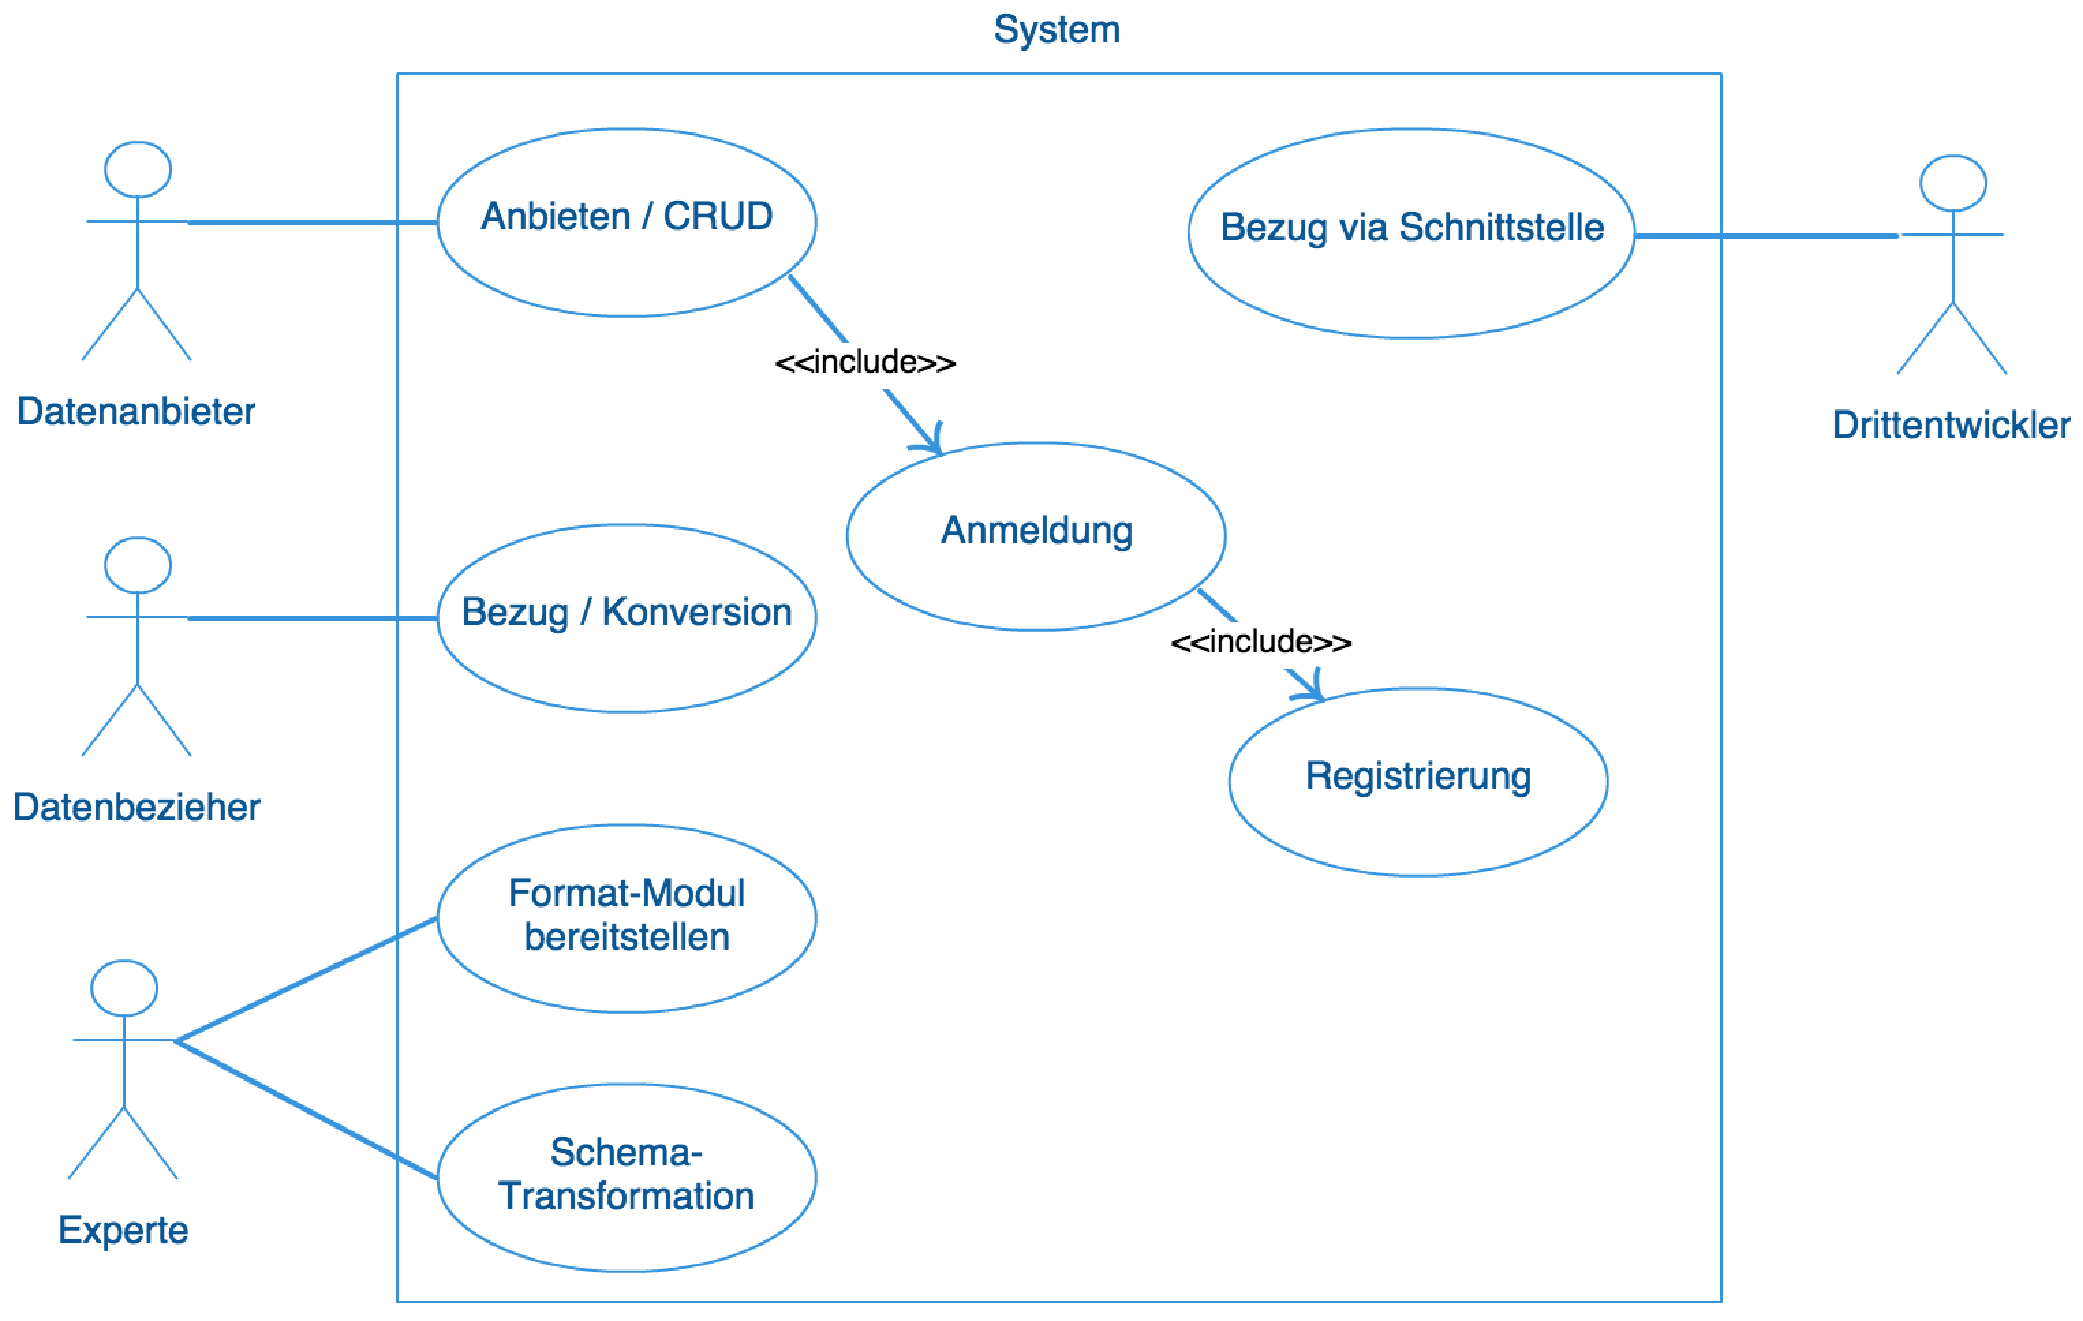
\includegraphics[width=0.9\linewidth]{fig/uc-diagramm}
	\caption{Übersicht Anforderungen}
	\label{fig:pd:uc-diagramm}
\end{figure}

\subsection{Konkrete Anwendungsfälle}
\label{sec:pd:usecases}

\subsubsection{Post- und Gebäudeadressen}
Adressen im Allgemeinen können auf unterschiedliche Art und Weise modelliert und abgespeichert werden. Das klassische Beispiel ist die Adresse inklusive Hausnummer gegenüber zwei separaten Feldern. Ziel wäre es unterschiedliche Schemata von Postadressen als integriertes zu \acs{csv} generieren, oder vorhandene Gebäudeadressen mit Daten im \gls{mopublic}\footnote{\url{http://www.cadastre.ch/internet/cadastre/en/home/products/mopublic.html}} Format anreichern zu können.

\subsubsection{Verkehrshindernisse}
Die Webapplikation \gls{trobdb} stellt Verkehrshindernisse der Schweiz auf einer Karte dar. Diese Verkehrshindernisse werden von diversen Datenlieferanten in unterschiedlichen Datei- und Schemaformaten angeliefert. Ziel ist es, alle diese Verkehrshindernisse in einem einheitlichen Datei- und Schemaformat beziehen zu können.

Als Datenquellen dienen Datenangebote des Bundes, der Kantone sowie Lichtenstein. Als Demonstration sollen folgende Datenquellen verwendet werden:
\begin{itemize}
\item Daten von \purl{http://www.truckinfo.ch} in einem nicht weiter spezifizierten XML-Format (siehe \cref{src:pd:truckinfoxml})
\item WFS des Kantons Zürich (Tiefbaustellen, Baustellen)
\item Excel-Datei des Kantons Appenzell Ausserrhoden
\item Für Google Earth erstelltes KML des Kantons Zürich
\end{itemize}

\begin{srclst}[label=src:pd:truckinfoxml]{xml}{XML von truckinfo.ch}
<evts>
<evt df="1430449200" dd="1430157600" r="A1" p="Switzerland" t="2" c="517" lar="3.7" cat="1_38" s="-1" x="539007" y="5257837" i="mapserver2/symbols/icone35.png">
[Switzerland] contraflow |Zurich - St. Margrethen|between junction St. Gallen-Kreuzbleiche and junction St. Gallen-Neudorf in both directions contraflow, temporary width limit 3.7 metres, set of roadworks during the night, length of the route affected: 3.7 km, speed limit: 80 km/h, duration: April 27, 2015 08:00 pm until May 01, 2015 05:00 am|
</evt>
<evt df="1430794800" dd="1430762400" r="A1" p="Switzerland" t="2" c="503" lar="6" cat="1_38" s="-1" x="533526" y="5257414" i="mapserver2/symbols/icone35.png">
[Switzerland] left lane(s) closed|St. Gallen - St. Margrethen|between junction St. Gallen-St. Fiden and junction St. Gallen-Neudorf in both directions left lane closed, temporary width limit 6.0 metres, set of roadworks during the night, length of the route affected: 1.3 km, speed limit: 80 km/h, duration: May 04, 2015 08:00 pm until May 05, 2015 05:00 am|
</evt>
<!-- ... -->
</evts>
\end{srclst}

\subsection{Rollen}
In \cref{tab:pd:rollen} sind die für das Projekt relevanten Rollen bzw. Akteure aufgelistet. Diese werden in den nachfolgenden Abschnitten referenziert.

\mytable{lX}{
	\textbf{Rolle} & \textbf{Beschreibung}\\
	\midrule

	\textbf{Datenanbieter} & Ist diejenige Person oder gar Unternehmen/Behörde die daran interessiert ist, eigene Daten zur Verfügung zu stellen ohne sich um dessen Format oder Schnittstellen zum Bezug kümmern zu müssen.\\

	\textbf{Schema-/Format-Experte} & Ist oftmals ein Datenanbieter selbst bzw. eine Person innerhalb dessen Organisation. Kann Schema-Transformationen mit OpenDataHub durchführen und ist dafür zuständig dem Administrator von OpenDataHub allfällige Module zur Unterstützung deren Format(e) innerhalb der Applikation zu liefern.\\

	\textbf{Datenbezieher} & Der Datenbezieher ist lediglich an einzelnen angebotenen Daten interessiert und möchte diese für eigene Zwecke weiterverwenden.\\

	\textbf{Drittentwickler} & Andere Entwickler welche die Funktionalität der Applikation via \acs{rest} \acs{api} nutzen wollen.\\

	\textbf{Administrator} & Der Applikationsverantwortliche, welcher die Applikation betreibt und wartet.\\
}{Rollen/Akteure}{pd:rollen}


\subsection{Registrierung / Authentifizierung}

\begin{scrumepic}[label=epic:pd:registrieren]{Benutzer registrieren}
	Als Datenanbieter will ich mich in der Applikation registrieren können, sodass ich Daten unter meiner Person/Organisation publizieren kann.
\end{scrumepic}

\begin{scrumstory}[label=story:pd:suisseid]{SuisseID}
	Als Datenanbieter will ich mich mittels SuisseID registrieren/anmelden können, sodass ich als Behörde einen Zugriff erlange ohne einen Social-Account zu benötigen.
\end{scrumstory}

\begin{scrumstory}[label=story:pd:github]{GitHub}
	Als Datenanbieter oder Drittentwickler will ich mich mittels GitHub-Konto registrieren/anmelden können, sodass ich Daten publizieren kann ohne ein separates Konto zu benötigen.
\end{scrumstory}

\begin{scrumstory}[label=story:pd:facebook]{Facebook}
	Als Datenanbieter oder Drittentwickler will ich mich mittels Facebook-Konto registrieren/anmelden können, sodass ich Daten publizieren kann ohne ein separates Konto zu benötigen.
\end{scrumstory}


\subsection{Daten publizieren}

\begin{scrumepic}[label=epic:pd:publizieren]{Daten publizieren}
	Als Datenanbieter will ich die Daten in diversen strukturierten Formaten anbieten können, sodass ich diese der Öffentlichkeit ohne zusätzlichen Aufwand bereitstellen kann.
	\storyacceptance	
	Gegeben
	\storyitem{eine oder mehrere Dateien in einem von der Applikation unterstützten Format}
	wenn der Datenanbieter die Datei via Webapplikation publiziert, dann soll diese in OpenDataHub abgespeichert werden und in einer Liste von verfügbaren Daten ersichtlich sein.
\end{scrumepic}

\begin{scrumstory}[label=story:pd:hochladen]{Datei hochladen}
	Als Datenanbieter will ich eine oder mehrere Dateien in einem strukturierten Format via Browser hochladen können, sodass ich diese auf der Plattform weiterverwenden kann.
\end{scrumstory}

\begin{scrumstory}[label=story:pd:online-quelle]{Online Quellen}
	Als Datenanbieter will ich Daten in einem strukturierten Format mit Angabe einer Online-Quelle (HTTP, WFS) publizieren können, sodass ich diese auf der Plattform weiterverwenden kann.
	\storyacceptance	
	Gegeben
	\storyitem{Daten sind Online in einem von der Applikation unterstützten Format verfügbar}
	wenn ich die Daten publiziere, dann sollen diese von der Applikation automatisch aus der angegebenen Quelle in die Applikation geladen werden und zur Verfügung stehen.
\end{scrumstory}

\begin{scrumstory}[label=story:pd:private-daten]{Private Daten}
	Als Datenanbieter will ich Daten als ``Privat'' markieren können, sodass diese nur von mir ersichtlich und beziehbar sind und nicht der Öffentlichkeit zur Verfügung stehen.
	\storyacceptance	
	Gegeben
	\storyitem{Dem Formular zur Publikation von Daten}
	wenn ich den Eintrag als Privat markiere, dann sollen die Daten für anonyme oder andere Benutzer nicht (mehr) in der Liste von verfügbaren Daten gelistet sein und jeglicher Zugriff darauf verweigert werden.
\end{scrumstory}

\begin{scrumstory}[label=story:pd:parser]{Modul anbieten}
	Als Datenanbieter bzw. Schema/Format-Experte will ich Python-Module (Plugins) welche eine gegebene Schnittstelle implementieren, anbieten, um die bereitgestellten Daten/Formate unterstützen zu können.
	\storyacceptance	
	Gegeben
	\storyitem{Einer vordefinierten Schnittstelle zur Programmierung eines solchen Moduls,}
	\storyitem{einem Beispiel eines solchen Moduls}
	wenn ein solches Modul bereitgestellt wird, dann soll das Format von der Applikation unterstützt werden.
\end{scrumstory}


\subsection{Daten transformieren}

\begin{scrumepic}[label=epic:pd:transformation]{Transformation}
	Als Experte will ich Transformationen mittels einer vorgegebenen Sprache oder Konfiguration erstellen können, sodass diverse heterogene Daten homogenisiert und in einem einheitlichen Format bezogen werden können.
	\storyacceptance	
	Gegeben
	\storyitem{Einer dokumentierten Schema-Mapping-Sprache oder -Konfiguration,}
	\storyitem{einem Beispiel eines solchen Mappings/Transformation,}
	wenn ich eine solche Transformation an die Applikation übergebe, dann soll diese auf die ausgewählten Daten angewendet werden. Das Resultat will ich analog wie einzelne Daten in \cref{epic:pd:datenbezug} in diversen Formaten beziehen können.
\end{scrumepic}

\begin{scrumstory}[label=story:pd:views]{Transformation publizieren}
	Als Experte will ich diese Transformationen (``Views'' auf die Daten) analog wie die einzelnen Daten speichern und publizieren können, sodass diese einerseits immer wieder per Knopfdruck angewendet und andererseits auch von anderen, nicht-Experten verwendet werden können.
\end{scrumstory}



\subsection{Daten beziehen}

\begin{scrumepic}[label=epic:pd:datenbezug]{Datenbezug}
	Als Endbenutzer will ich die bereitgestellten Daten in einem von mir gewünschten, strukturierten Format beziehen können.
	\storyacceptance	
	Gegeben
	\storyitem{Eine in der Applikation von einem Datenanbieter abgelegten Datei,}
	\storyitem{eine Datei dessen Format von der Applikation unterstützt wird,}
	wenn ich die Datei mittels Browser in einem anderen Format beziehen will, dann soll die automatisch ins Zielformat konvertierte Datei heruntergeladen werden.
\end{scrumepic}



\section{Nicht-funktionale Anforderungen}
%(Rahmenbedingungen, evtl. Verweis auf 1.3)

Die nicht-funktionalen Anforderungen der einzelnen User Stories sind grundsätzlich in deren Akzeptanzkriterien enthalten.
In diesem Abschnitt werden zusätzliche, aus der Aufgabenstellung entnommene sowie bei dem Betreuer aufgenommene nicht-funktionale Anforderungen, ergänzt durch sinnvolle Anforderungen moderner Software-Entwicklung beschrieben.

\subsection{Technologien}
Die Anforderungen an die eingesetzten Technologien\footnote{Programmiersprachen, Frameworks, Libraries, Services, \dots} sind teilweise durch die Aufgabenstellung sowie durch die bereits existierende Infrastruktur am Geometa Lab der HSR wie folgt eingeschränkt:

\begin{itemize}
	\item Python als Programmiersprache
	\item Deployment der Applikation muss via \gls{wsgi} möglich sein
	\item \gls{psql} als Datenbank oder SQLite bei kleineren Aufgaben
\end{itemize}


Die Wahl der Frameworks und Libraries, sowohl Server- wie auch Clientseitig ist dem Entwicklerteam überlassen.

\subsection{Qualität}
Zur Sicherung der Softwarequalität wurden folgende drei Anforderungen durch den Betreuer bestimmt:

\begin{itemize}
	\item Einsatz von automatisierten Unit Tests
	\item Kommentieren des Codes in einem Sphinx\footnote{Siehe auch: \url{http://sphinx-doc.org}} kompatiblen Format
	\item PEP-8 als Codierrichtlinie, besonders die Verwendung von Leerzeichen zur Einrückung
\end{itemize}


\subsection{Effizienz}
Bei der Applikation handelt es sich einerseits um einen Prototypen, andererseits nicht um eine Echtzeit-Applikation. Dennoch sollte die Applikation mit Datenmengen von maximal 500000 Datensätzen umgehen können, sofern genügend Arbeitsspeicher vorhanden ist.



